%%%%%%%%%%%%%%%%%%%%%%%%%%%%%%%%%%%%%%%%%
% University Assignment Title Page 
% LaTeX Template
% Version 1.0 (27/12/12)
%
% This template has been downloaded from:
% http://www.LaTeXTemplates.com
%
% Original author:
% WikiBooks (http://en.wikibooks.org/wiki/LaTeX/Title_Creation)
%
% License:
% CC BY-NC-SA 3.0 (http://creativecommons.org/licenses/by-nc-sa/3.0/)
% 
% Instructions for using this template:
% This title page is capable of being compiled as is. This is not useful for 
% including it in another document. To do this, you have two options: 
%
% 1) Copy/paste everything between \begin{document} and \end{document} 
% starting at \begin{titlepage} and paste this into another LaTeX file where you 
% want your title page.
% OR
% 2) Remove everything outside the \begin{titlepage} and \end{titlepage} and 
% move this file to the same directory as the LaTeX file you wish to add it to. 
% Then add \input{./title_page_1.tex} to your LaTeX file where you want your
% title page.
%
%%%%%%%%%%%%%%%%%%%%%%%%%%%%%%%%%%%%%%%%%
%\title{Title page with logo}
%----------------------------------------------------------------------------------------
%	PACKAGES AND OTHER DOCUMENT CONFIGURATIONS
%----------------------------------------------------------------------------------------

\documentclass[12pt]{article}
\usepackage[margin=1in]{geometry}
\usepackage[english]{babel}
\usepackage{url}
\usepackage[utf8x]{inputenc}
\usepackage{amsmath}
\usepackage{graphicx}
\usepackage[colorinlistoftodos]{todonotes}
\usepackage[sort, numbers]{natbib}
\graphicspath{img/}

\usepackage{caption}
\DeclareCaptionFormat{citation}{%
   \ifx\captioncitation\relax\relax\else
     \captioncitation\par
   \fi
   #1#2#3\par}
\newcommand*\setcaptioncitation[1]{\def\captioncitation{\textit{Image source:}~#1}}
\let\captioncitation\relax
\captionsetup{format=citation,justification=centering}

\begin{document}

\begin{titlepage}

\newcommand{\HRule}{\rule{\linewidth}{0.5mm}} % Defines a new command for the horizontal lines, change thickness here

\center % Center everything on the page
 
%----------------------------------------------------------------------------------------
%	HEADING SECTIONS
%----------------------------------------------------------------------------------------

\textsc{\LARGE Ukrainian Catholic University}\\[1cm] % Name of your university/college
\textsc{\Large Applied Sciences Faculty}\\[0.5cm] % Major heading such as course name
\textsc{\large Data Science Master Programme}\\[0.5cm] % Minor heading such as course title

%----------------------------------------------------------------------------------------
%	TITLE SECTION
%----------------------------------------------------------------------------------------

\HRule \\[0.4cm]
{ \huge \bfseries Abstractive text summarization with Recurrent Neural
	Networks}\\[10pt]
{\Large \bfseries Machine Learning project report}\\[0.4cm] % Title of your document
\HRule \\[1cm]
 
%----------------------------------------------------------------------------------------
%	AUTHOR SECTION
%----------------------------------------------------------------------------------------


% If you don't want a supervisor, uncomment the two lines below and remove the section above
\Large \emph{Authors:}\\
Hanna \textsc{Pylieva}\\Yuriy \textsc{Mykhalchuk}\\Irynei \textsc{Baran}\\[0.5cm] % Your name

%----------------------------------------------------------------------------------------
%	DATE SECTION
%----------------------------------------------------------------------------------------

{\large \today}\\[2cm] % Date, change the \today to a set date if you want to be precise

%----------------------------------------------------------------------------------------
%	LOGO SECTION
%----------------------------------------------------------------------------------------


\includegraphics[height=4cm]{img/UCU-Apps.png}\\[1cm] % Include a department/university logo - this will require the graphicx package
 
%----------------------------------------------------------------------------------------

\vfill % Fill the rest of the page with whitespace

\end{titlepage}


\begin{abstract}
\todo[inline, color=green!40]{Invent a meaningful abstract.}In this work, we cast text summarization as a sequence-to-sequence problem and apply the attentional encoder-decoder RNN that has been shown to be successful for Neural Machine Translation \cite{baseline_NMT}.
\end{abstract}

\section{Introduction}

\todo[inline, color=green!40]{Invent a meaningful introduction. Per Shelpuk: Good project will be dedicated to an important problem and have a clear vision of what value it can bring to the potential users. All stages will be explored and analyzed, the approach for each of them is selected thoughtfully, compared to the alternatives and clearly explained. The results are evaluated and explained (explanation should provide additional information, not just restating the results or the code in English).}
In the modern Internet age, textual data is ever increasing. According to this each Internet user will highly benefit from condensing data while preserving the information and meaning. This idea is a driver of growing interest among the research community for developing new approaches to automatically summarize the text. Automatic text summarization system generates a short summary that captures the main ideas
of an input text. Since the advent of text summarization in 1950s, researchers have been trying to improve techniques for generating machine summaries which are not worse than human made summaries \cite{text_sum_survey}.
  
There are two prominent types of summarization algorithms.

\begin{itemize}
	\item Extractive summarization copies parts of the source text through some measure of importance and then combines those part/sentences together to render a summary. Importance of sentence is based on linguistic and statistical features.

	\item Abstractive summarization generates new phrases, possibly rephrasing or using words that were not in the original text. Naturally abstractive approaches are harder as it involves robust natural language processing. For perfect abstractive summary, the model has to first understand the document and then express that understanding in succinct form possibly using new words and phrases.  Abstractive summarization has complex capabilities like generalization, paraphrasing and incorporating  real-world knowledge \cite{abstractive_text_summarization}.
\end{itemize}

Majority of the work has traditionally focused on extractive approaches due to the easy of defining hard-coded rules to select important sentences than generate new ones. Also, it promises grammatically correct and coherent summary. But they often don’t summarize long and complex texts well as they are very restrictive.


Abstractive methods, on the other hand, provide highly powerful and promising results. That is why in this project we implemented an algorithm for abstractive text summarization to build solid understanding if this approach and discover how it can be improved.


\section{Model}
\subsection{Background}
Models for abstractive text summarization fall under a larger deep learning category called
sequence-to-sequence models, which map from an input sequence to a target sequence. This approach is illustrated on Figure~\ref{fig:seq-to-seq}. It was initially used for Neural Machine Translation as described in \cite{attention_based_NMT}. 


\begin{figure}[h]
	\centering
	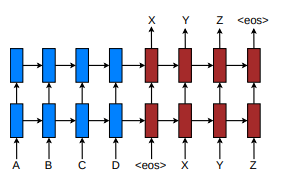
\includegraphics[width=0.5\textwidth]{img/seq-to-seq.png}
	\setcaptioncitation{\cite{attention_based_NMT}}
	\caption{\label{fig:seq-to-seq}The model reads an input sentence “ABC” and produces “WXYZ” as the output 	sentence. The model stops making predictions after outputting the $<$eos$>$ token. It then starts 		 emiting one target word at a time. }
\end{figure}


An effective and standard approach to build sequence-to-sequence models is using Encoder-Decoder architecture that act as an encoder and a decoder pair. The encoder reads the entire input sequence and encodes it into an internal representation, often a fixed-length vector called the context vector. The decoder reads the encoded input sequence and generates the output sequence. Both the encoder and the decoder submodels are trained jointly, i.e. at the same time.

Naturally we need the input and output to be of variable-length. This can not be reached with ordinary Deep Neural Networks (DNNs) which require that the dimensionality of the inputs and outputs is known and fixed. 

The Recurrent Neural Networks (RNNs) are generalization of feedforward neural networks to sequences. Given a sequence of inputs $(x_1, ..., x_T)$, a standard RNN computes a
sequence of outputs $(y_1, ..., y_T)$ by iterating the following equation \cite{seq2seq_with_NN} :

\begin{equation}
\begin{array}{l}
	h_t = f(W^{hx}x_t + W^{hh}h_{t-1}) \\
	y_t = W^{yh}h_t
\end{array}
\end{equation}
where 
$f$ - activation function,
$x_{t}$ - input vector, 
$h_{t}$ - hidden layer vector,
$y_{t}$ - output vector,
$W$ - parameter matrix
 
 
An RNN can map sequences to sequences provided that the alignment between the inputs the
outputs is known ahead. In other words RNN needs a defined one-to-one correspondence between a sequence of inputs and sequence of outputs which can be understood better from RNN unfold representation on Figure~\ref{fig:RNN}.

\begin{figure}[h]
	\centering
	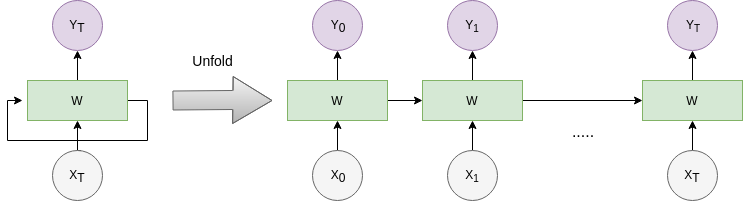
\includegraphics[width=0.8\textwidth]{img/RNN.png}
	\setcaptioncitation{Created by author}
	\caption{\label{fig:RNN}Recurrent Neural Network}
\end{figure}
 
However, it is not clear how to apply an RNN to problems whose input and the output sequences have different lengths with complicated and non-monotonic relationships.

The simplest strategy for general sequence learning is to map the input sequence to a fixed-sized
vector using one RNN, and then to map that vector to the target sequence with another RNN (the
approach is represented in \cite{baseline_NMT}). Since the RNN is provided with all the relevant information this will work. Whereas the need to store information over extended time interval will lead to difficulties with training RNN (vanishing gradient problem/exploding gradientt problem explained in \cite{LSTM_baseline}).
Here Long Short-Term Memory (LSTM) layers will come in handy as they are known to learn problems with long range temporal dependencies and will succeed in this setting.

\subsubsection{LSTM}

The goal of LSTM in general is to estimate the conditional probability of outpuy sequence by input sequence $p(y_1, ..., y_{T′}|x_1, ..., x_T )$ when lengths of those sequences are possibly: $T' \neq T$. 
An LSTM computes this conditional probability by first obtaining the fixed dimensional
representation $v$ of the input sequence $(x_1, ..., x_T)$ given by the last hidden state of the LSTM, and then computing the probability of $y_1, ..., y_{T′}$ with a standard LSTM-LM
\footnote{Language Model (LM) is a probability distribution over sequences of words. LSTM-LM is algorithm of using an LSTM (and softmax function) to predict the next word given your previous words.} 
formulation whose initial hidden state is set to the representation $v$ of  $x_1, ..., x_T$:

$$p(y_1, ..., y_{T′}|x_1, ..., x_T ) = \prod_{t=1}^{T'} p(y_t|v, y_1, ..., y_{t-1}) $$


In this equation, each $p(y_t|v, y_1, ..., y_{t-1})$ distribution is represented with a softmax over all the
words in the vocabulary \cite{seq2seq_with_NN}.

Taking into consideration all above and having processed prominent researches on abstractive summarization topic we've built an encoder-decoder recurrent neural network with LSTM units and attention mechanism to generate headlines from the text of news articles. We took the model described in \cite{basic-article} as baseline, but performed some modifications according to available software restrictions.

\subsection{Overview}
In our model encoder and decoder get more precise descriptions. 

\subsubsection{Encoder}
The input of encoder (Figure~\ref{fig:encoder}) consists of article's text of restricted size followed by an end-of-sequence symbol ($w_{EOS}$, in code we used '$<>$') followed by header. Each word of input is first passed through an embedding layer which transforms it into a distributed representation. So now each word has a corresponding vector $w \in R^d$.
In our case encoder consists of 2 LSTMs, both on hidden layer. We run the stacked LSTMs over the sequence of vectors and store the last hidden state - this is encoder representation $e$, which will be used to generate by decoder to generate the target sequence word by word.   

%\begin{figure}[h]
%\centering
%	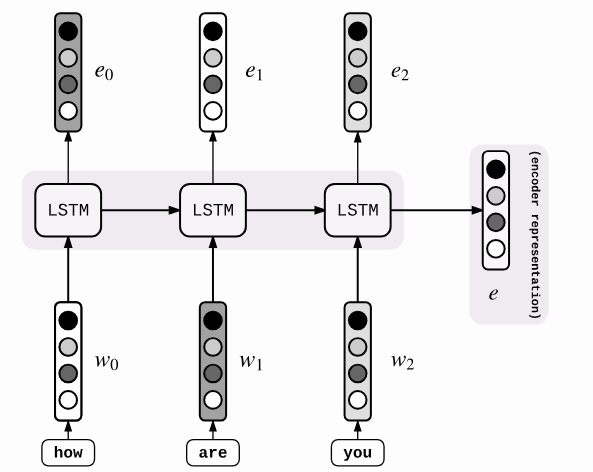
\includegraphics[width=0.45\textwidth]{img/seq2seq_vanilla_encoder.png}
%	\setcaptioncitation{\url{https://guillaumegenthial.github.io/sequence-to-sequence.html}}
%	\caption{\label{fig:encoder}LSTM-based Encoder}
%\end{figure}

\subsubsection{Decoder}
\todo{Does this section looks ok with index 0 in the beginning and t in the end?}
Our decoder consist of 1 LSTM cell. We feed $e$ as  hidden state and $w_{eos}$ symbol into decoder as input. The LSTM computes the next hidden state $h_0 \in R^h$. Then a function $f: R^h \rightarrow R^V$ is applied so that $s_0 := g(h_0) \in R^V$ is a vector of the same size as vocabulary. Then a softmax is applied to $s_0$ to normalize it into a vector of likelihood of each word in the vocabulary being the next word in the sequence. The task of decoder is to find the most likely output sequence. Due to big vocabulary size the search problem through all the possible output sequences based on their likelihood is exponential in length of the output sequence and is NP-complete. That is why it is common to use approximate methods. We used beam search and were keeping in memory 10 best output sequences (hypotheses) to eventually opt for the best combination of words. On each step after we've found the index $i_t$ of the desired word, we get a vector $w_{i_t}$ corresponding to it and repeat the procedure: LSTM is fed with the hidden state $h_t$ and a word $w_{i_t}$, it will output the next word in output sequence. The process repeats until $w_{eos}$ is generated.

\begin{figure}[h]
\centering
	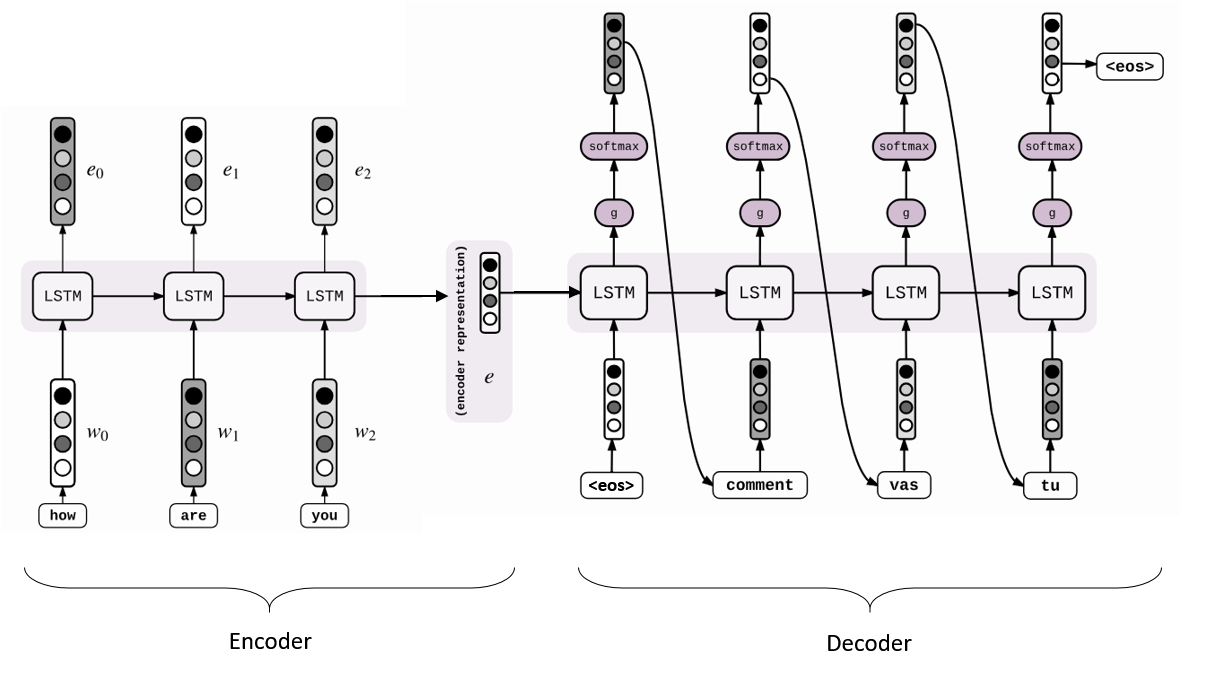
\includegraphics[width=0.7\textwidth]{img/seq2seq-detailed1.png}
	\setcaptioncitation{\url{https://guillaumegenthial.github.io/sequence-to-sequence.html}}
	\caption{\label{fig:encoder}LSTM-based sequence to sequence model}
\end{figure}

The described process corresponds to testing phase. On training phase instead of feeding in as input of new generative step the freshly generated word, the expected word from the actual headline is fed in. This leads to a disconnect between training
and testing. To overcome this disconnect, during training we randomly feed in a generated word,
instead of the expected word, as suggested in \cite{scheduled_sampling}. Specifically, we do this for 10\% of cases. This approach is called "teacher forcing".


%\begin{equation}
%\begin{array}{l}
%	h_0 = LSTM(e, [w_{eos}, c_t]) \\
%	s_0 = g(h_0) \\
%	p_0 = softmax(s_0)\\
%	i_0 = argmax(p_0)\\
%	
%	t = 1\\
%	while \; w_{i{t-1}} \neq w_{eos}:\\
%\quad		h_t = LSTM(e, [w_{i{t-1}}, c_t])\\
%\quad		s_t = g(h_t)\\
%\quad		p_t = softmax(s_t)\\
%\quad		i_t = argmax(p_t)\\
%\quad		t += 1	\\
%\end{array}
%\end{equation}


\subsubsection{Attention} \label{attention}
Attention is a mechanism that addresses a limitation of the encoder-decoder architecture on long sequences, and that in general speeds up the learning and lifts the skill of the model on sequence to sequence prediction problems. The attention mechanism is used when outputting each word in the decoder. For each output word the attention mechanism computes a weight over each of the input
words that determines how much attention should be paid to that input word. The weights sum up to
1, and are used to compute a weighted average of the last hidden layers generated after processing
each of the input words. This weighted average, referred to as the context, is then input into the
softmax layer along with the last hidden layer from the current step of the decoding.


\subsubsection{Training details}

\begin{thebibliography}{9}
	\bibitem{baseline_NMT}
	Bahdanau,D.; Cho,K.; Bengio Y. \textit{Neural machine translation by jointly learning to align and translate}. CoRR, abs/1409.0473, 2014. \url{ http://arxiv.org/abs/1409.0473}.
	
	\bibitem{text_sum_survey}
	Gambhir, M. and Gupta, V. \textit{Recent automatic text summarization techniques: a survey}. Artificial Intelligence Review, 47(1):1-66, 2017.
	
	\bibitem{abstractive_text_summarization}
	Singhal,S. and Bhattacharya, A. \textit{Abstractive Text Summarization}. Department of Computer Science IIT Kanpur, 2017.
	
	\bibitem{attention_based_NMT}
	Minh Thang Luong; Hieu Pham; Christopher D. Manning. \textit{Effective Approaches to Attention-based Neural Machine Translation}. CoRR, abs/1508.04025, 2015. \url{http://arxiv.org/abs/1508.04025}
	
	\bibitem{seq2seq_with_NN}
	Ilya Sutskever, Oriol Vinyals, Quoc V. Le \textit{Sequence to Sequence Learning with Neural Networks}. CoRR, abs/1409.3215, 2014. \url{http://arxiv.org/abs/1409.3215}
	
	\bibitem{LSTM_baseline}	
	S. Hochreiter and J. Schmidhuber. \textit{Long short-term memory}. Neural Computation, 1997.
		 
	\bibitem{basic-article}
	Lopyrev, K.\textit{Generating News Headlines with Recurrent Neural 	Networks}. CoRR, abs/1512.01712, 2015.
	
	\bibitem{scheduled_sampling}
	Samy Bengio, Oriol Vinyals, Navdeep Jaitly, and Noam Shazeer. \textit{Scheduled sampling for sequence
prediction with recurrent neural networks}. CoRR, abs/1506.03099, 2015. \url{http://arxiv.org/abs/1506.03099}
	
%	\bibitem{deep_learning_basic}
%	Ian Goodfellow, Yoshua Bengio, Aaron Courville \textit{Deep Learning}. MIT Press. 2016. \url{http://www.deeplearningbook.org/}
	
%	\bibitem{bishop}
%	Bishop, Christopher M.	\textit{Pattern Recognition and Machine Learning}. %Springer, Cambridge, U.K., 2006.

\end{thebibliography}


\end{document}